\section{Browser-Technologien}

\subsection{Vordefinierte Objekte}
\begin{concept}{Browser-Objekte}
Browser-Objekte existieren auf der Browser-Plattform und beziehen sich auf verschiedene Aspekte wie das Browser-Fenster, das angezeigte Dokument oder den Browser selbst. Beispiele sind:
\begin{itemize}
  \item \textbf{Document:} Zugriff auf das DOM (Document Object Model) der aktuellen Webseite.
  \item \textbf{Window:} Repräsentiert das Browserfenster und bietet globale Funktionen.
  \item \textbf{Navigator:} Informationen über den Browser und das Gerät.
  \item \textbf{Location:} Zugriff auf die aktuelle URL und zugehörige Methoden.
\end{itemize}
\end{concept}

\begin{definition}{Document}
Das \texttt{document}-Objekt repräsentiert die angezeigte Webseite und bietet diverse Attribute und Methoden:
\begin{lstlisting}[language=JavaScript, style=basesmol]
document.cookie          // Zugriff auf Cookies
document.lastModified    // Zeitpunkt der letzten anderung
document.links           // Verweise auf der Seite
document.images          // Bilder auf der Seite
\end{lstlisting}
\end{definition}

\begin{definition}{Window}
Das \texttt{window}-Objekt repräsentiert das Browserfenster. Es bietet Zugriff auf:
\begin{itemize}
  \item Globale Variablen und Methoden (z.B. \texttt{setTimeout, alert}).
  \item Fensterattribute (z.B. \texttt{innerHeight, pageYOffset}).
  \item Das DOM der aktuellen Seite (\texttt{window.document}).
\end{itemize}
\begin{lstlisting}[language=JavaScript, style=basesmol]
window.document /* Zugriff auf Dokument */
window.history /* History-Objekt */
window.innerHeight /* height of Viewport */
window.pageYOffset /* vertikal gescrollte Pixel */
window.alert === alert /* -> true */
window.setTimeout === setTimeout /* -> true */
window.parseInt === parseInt /* true */
\end{lstlisting}
\end{definition}

\begin{definition}{Navigator}
Das \texttt{navigator}-Objekt liefert Informationen über den Browser und das Gerät:
\begin{lstlisting}[language=JavaScript, style=basesmol]
console.log(navigator.userAgent)  // Browser-Details
console.log(navigator.language)   // Spracheinstellung
console.log(navigator.onLine)     // Online-Status
\end{lstlisting}
\end{definition}

\begin{definition}{Location}
Das \texttt{location}-Objekt bietet Zugriff auf die URL der aktuellen Seite:
\begin{lstlisting}[language=JavaScript, style=basesmol]
console.log(location.href)       // Vollstandige URL
location.reload()                // Seite neu laden
\end{lstlisting}
\end{definition}

\subsection{DOM (Document Object Model)}

\begin{code}{DOM-Manipulation}
\begin{lstlisting}[language=JavaScript, style=basesmol]
let aboutus = document.getElementById("aboutus")
let links = aboutus.querySelectorAll("a")
links.forEach(link => {
    console.log(link.href)
})
\end{lstlisting}

\begin{lstlisting}[language=JavaScript, style=basesmol]
document.createElement    // Element erzeugen
document.createAttribute  // Attribute erzeugen
document.setAttribute     // Und hinzufugen
document.appendChild      // Element in Baum einfugen
\end{lstlisting}
\end{code}

\begin{examplecode}{Elemente auffinden}
\begin{lstlisting}[language=JavaScript, style=basesmol]
let aboutus = document.getElementById("aboutus")
let aboutlinks = aboutus.getElementsByTagName("a")
let aboutimportant = aboutus.getElementsByClassName("important")
let navlinks = document.querySelectorAll("nav a")
\end{lstlisting}
\end{examplecode}
  
\begin{examplecode}{Textknoten erzeugen}
\begin{lstlisting}[language=JavaScript, style=basesmol]
<p>The <img src="img/cat.png" alt="Cat"> in the
<img src="img/hat.png" alt="Hat">.</p>
<p><button onclick="replaceImages()">Replace</button></p>
<script>
  function replaceImages () {
    let images = document.body.getElementsByTagName("img")
    for (let i = images.length - 1; i >= 0; i--) {
      let image = images[i]
      if (image.alt) {
      let text = document.createTextNode(image.alt)
      image.parentNode.replaceChild(text, image)
      }
    }
  }
</script>
\end{lstlisting}
\end{examplecode}


  
\begin{examplecode}{Elementknoten erzeugen}
\begin{lstlisting}[language=JavaScript, style=basesmol]
<blockquote id="quote">
  No book can ever be finished. While working on it we learn ...
</blockquote>
<script>
/* definition of elt ... */
document.getElementById("quote").appendChild(
  elt("footer", "-",
  elt("strong", "Karl Popper"),
  ", preface to the second edition of ",
  elt("em", "The Open Society and Its Enemies"),
  ", 1950"))
</script>
\end{lstlisting}
\end{examplecode}
  
\begin{examplecode}{Attribut setzen}
\begin{lstlisting}[language=JavaScript, style=basesmol]
let h1 = document.querySelector("h1")

let att = document.createAttribute("class")
att.value = "democlass"
h1.setAttributeNode(att)

/* in short: */
h1.setAttribute("class", "democlass")
\end{lstlisting}
\end{examplecode}

\begin{examplecode}{Style anpassen}
\begin{lstlisting}[language=JavaScript, style=basesmol]
<p id="para" style="color: purple">Nice text</p>
<script>
  let para = document.getElementById("para")
  console.log(para.style.color)
  para.style.color = "magenta"
</script>
\end{lstlisting}
\end{examplecode}
  
\columnbreak

\subsection{Event-Handling}

\begin{formula}{Event Handling}
Ereignisse wie Mausklicks oder Tastatureingaben können mit Event-Handlern behandelt werden:
\begin{lstlisting}[language=JavaScript, style=basesmol]
let button = document.querySelector("button")
button.addEventListener("click", () => {
    console.log("Button geklickt!")
})
\end{lstlisting}
\end{formula}

\begin{code}{Event abonnieren/entfernen}
  Mit der Methode addEventListener() wird ein Event abonniert. Mit removeEventListener kann das Event entfernt werden.
\begin{lstlisting}[language=JavaScript, style=basesmol]
<button>Act-once button</button>
<script>
  let button = document.querySelector("button")
  function once () {
    console.log("Done.")
    button.removeEventListener("click", once)
  }
  button.addEventListener("click", once)
</script>
\end{lstlisting}
\end{code}
  
\begin{code}{Event-Objekt}

Wenn ein Parameter zur Methode hinzugefügt wird, wird dieses als das Event-Objekt gesetzt.
\begin{lstlisting}[language=JavaScript, style=basesmol]
<script>
    let button = document.querySelector("button")
    button.addEventListener("click", (e) => {
        console.log("x="+e.x+", y="+e.y)
    })
</script\
\end{lstlisting}
\end{code}

\begin{examplecode}{stopPropagation()}

Das Event wird bei allen abonnierten Handlern ausgeführt bis ein Handler stopPropagation() ausführt.
\begin{lstlisting}[language=JavaScript, style=basesmol]
<script>
  let button = document.querySelector("button")
  button.addEventListener("click", (e) => {
    console.log("x="+e.x+", y="+e.y)
    e.stopPropagation()
  })
</script>
\end{lstlisting}
\end{examplecode}

\begin{examplecode}{preventDefault()}

Viele Ereignisse haben ein Default verhalten. Eigene Handler werden vor Default-Verhalten ausgeführt. Um das Default-Verhalten zu verhindern, muss die Methode preventDefault() ausgeführt werden.
\begin{lstlisting}[language=JavaScript, style=basesmol]
<a href="https://developer.mozilla.org/">MDN</a>
<script>
  let link = document.querySelector("a")
  link.addEventListener("click", event => {
    console.log("Nope.")
      event.preventDefault()
  })
,/script>
\end{lstlisting}
\end{examplecode}

\begin{definition}{Tastatur-Events}
\texttt{keydown} (Achtung: kann mehrmals ausgelöst werden) und \texttt{keyup}:
\begin{lstlisting}[language=JavaScript, style=basesmol]
<p>Press Control-Space to continue.</p>
<script>
    window.addEventListener("keydown", event => {
            if (event.key ==" " && event.ctrlKey) {
                console.log("Continuing!")
            }
    })
</script>
\end{lstlisting}
\end{definition}

\begin{definition}{Maus-Events}
  
  \begin{minipage}{0.45\linewidth}
  \begin{itemize}
  \item Mausklicks:
  \begin{itemize}
    \item mousedown
    \item mouseup
    \item click
    \item dblclick
  \end{itemize}
  \end{itemize}
  \end{minipage}
  \begin{minipage}{0.5\linewidth}
    \begin{itemize}
    \item Mausbewegung
    \begin{itemize}
      \item mousemove
    \end{itemize}
    \item Touch-display
    \begin{itemize}
      \item touchstart
      \item touchmove
      \item touched
    \end{itemize}
    \end{itemize}
    \end{minipage}
\end{definition}


\begin{definition}{Scroll-Events}
Das Scrollevent enthält Attribute wie \texttt{pageYOffset} und \texttt{pageXOffset}.
\begin{lstlisting}[language=JavaScript, style=basesmol]
window.addEventListener("scroll", () => {
    let max = document.body.scrollHeight - window.innerHeight;
    let bar = document.querySelector("#scrollbar");
    bar.style.width = `${(window.pageYOffset / max) * 100}%`;
});
\end{lstlisting}
\end{definition}

\begin{definition}{Focus-Events}

Fokus- und Ladeereignisse
\begin{itemize}
  \item Fokus erhalten / verlieren
  \subitem focus
  \subitem blur
  \item Seite wurde geladen (ausgelöst auf window und document.body)
  \subitem load
  \subitem beforeunload
\end{itemize}
\end{definition}

\subsection{Jquery}
JQuery ist eine freie JavaScript-Bibliothek, die Funktionen zur DOM-Navigation und -Manipulation zur Verfügung stellt.

\begin{lstlisting}[language=JavaScript, style=basesmol]
$("button.continue").html("Next Step...")
var hiddenBox = $("#banner-message")
$("#button-container button").on("click", function(event) {
        hiddenBox.show()
    .})
\end{lstlisting}

\begin{definition}{\$(Funktion)} $\rightarrow$ DOM ready\\
\begin{lstlisting}[language=JavaScript, style=basesmol]
$(function() { 
  // Code to run when the DOM is ready
});
\end{lstlisting}
\end{definition}

\begin{definition}{\$("CSS Selektor").aktion(...)} $\rightarrow$ Wrapped Set\\
  Knoten, die Sel. erfüllen, eingepackt in ein jQuery-Objekt
\begin{lstlisting}[language=JavaScript, style=basesmol]
$(".toggleButton").attr("title");
// Get the title attribute of elements with class 'toggleButton'
\end{lstlisting}
\begin{lstlisting}[language=JavaScript, style=basesmol]
$(".toggleButton").attr("title", "click here");
// Set the title attribute of elements with class 'toggleButton' to 'click here'
\end{lstlisting}
\begin{lstlisting}[language=JavaScript, style=basesmol]
$(".toggleButton").attr({
  title: "click here",
  // other attributes
});
// Set multiple attributes of elements with class 'toggleButton'
\end{lstlisting}
\begin{lstlisting}[language=JavaScript, style=basesmol]
$(".toggleButton").attr("title", function() {
  // function to set title
}).css({
  // CSS properties
}).text("New Text").on("click", function(event) {
  // click event handler
});
\end{lstlisting}
\end{definition}

\begin{definition}{\$("HTML-Code")}$\rightarrow$ Create new elements (Wrapped Set)
  neuer Knoten erstellen und in ein jQuery-Objekt einpacken, noch nicht im DOM
\begin{lstlisting}[language=JavaScript, style=basesmol]
$("<li>...</li>").addClass("new-item").appendTo("ul");
// Create a new list item, add a class, and append it to a list
\end{lstlisting}
\begin{lstlisting}[language=JavaScript, style=basesmol]
$("<li>...</li>").length;
// Get the length of the new list item
\end{lstlisting}
\begin{lstlisting}[language=JavaScript, style=basesmol]
$("<li>...</li>")[0];
// Get the raw DOM element of the new list item
\end{lstlisting}
\end{definition}

\begin{definition}{Wrapped Set from DOM node}
  dieser Knoten in ein jQuery-Objekt eingepackt
\begin{lstlisting}[language=JavaScript, style=basesmol]
$(document.body);
// Wrap the body element in a jQuery object
\end{lstlisting}
\begin{lstlisting}[language=JavaScript, style=basesmol]
$(this);
// Wrap the current element in a jQuery object
\end{lstlisting}
\end{definition}

\subsection{Graphics}

\begin{definition}{Web-Grafiken}
\begin{itemize}
  \item Einfache Grafiken mit HTML und CSS möglich
  \item Zum Beispiel: Balkendiagramme
  \item Alternative für Vektorgrafiken: SVG
  \item Alternative für Pixelgrafiken: Canvas
\end{itemize}
\end{definition}

\subsubsection{SVG und Canvas}

\begin{definition}{SVG}
Scalable Vector Graphics
\begin{itemize}
  \item Basiert wie HTML auf XML
  \item Elemente repräsentieren grafische Formen
  \item Ins DOM integriert und durch Scripts anpassbar
\end{itemize}
\begin{lstlisting}[language=JavaScript, style=basesmol]
p>Normal HTML here.</p>
<svg xmlns="http://www.w3.org/2000/svg">
    <circle r="50" cx="50" cy="50" fill="red"/>
    <rect x="120" y="5" width="90" height="90" stroke="blue" fill="none"/>
</svg>
\end{lstlisting}
Ausgabe:\\
Normal HTML here.\\

\includegraphics[width=\linewidth]{images/2024_12_29_858f09cde51177c71657g-27}
\end{definition}

\begin{examplecode}{SVG mit JavaScript}
\begin{lstlisting}[language=JavaScript, style=basesmol]
let circle = document.querySelector("circle")
circle.setAttribute("fill","cyan")
\end{lstlisting}
\end{examplecode}


\begin{definition}{Canvas}
  Das \texttt{<canvas>}-Element bietet eine Zeichenfläche (API) für Pixelgrafiken:
\begin{lstlisting}[language=JavaScript, style=basesmol]
<canvas></canvas>
<script>
  Let cx = document.querySelector("canvas").getContext("2d")
  cx.beginPath()
  cx.moveTo(50, 10)
  cx.lineTo(10, 70)
  cx.lineTo(90, 70)
  cx.fill()
  let img = document.createElement("img")
  img.src = "img/hat.png"
  img.addEventListener("load" , () => {
      for (let x = 10; x < 200; x += 30) {
          cx.drawImage(img, x, 10)
      }
  })
</script>
\end{lstlisting}
\end{definition}


\begin{code}{Canvas Methoden}
  \begin{itemize}
    \item \texttt{scale} - Skalieren
    \item \texttt{translate} - Koordinatensystem verschieben
    \item \texttt{rotate} - Koordinatensystem rotieren
    \item \texttt{save} - Transformationen auf Stack speichern
    \item \texttt{restore} - Letzten Zustand wiederherstellen
  \end{itemize}  
\end{code}


\subsection{Browser-API}
Web Storage\\
Web Storage speichert Daten auf der Seite des Client.

\begin{definition}{Local Storage}
Mit \texttt{localStorage} können Daten auf dem Client gespeichert werden:
\begin{lstlisting}[language=JavaScript, style=basesmol]
localStorage.setItem("username", "Max")
console.log(localStorage.getItem("username")) // -> Max
localStorage.removeItem("username")
\end{lstlisting}
\end{definition}

\begin{definition}{Local Storage}
Local Storage wird verwendet, um Daten der Webseite lokal abzuspeichern. Die Daten bleiben nach dem Schliessen des Browsers erhalten. Die Daten sind in Developer Tools einsehbar und änderbar.

Die Daten werden nach Domains abgespeichert. Es können pro Webseite etwa 5MB abgespeichert werden.

\begin{lstlisting}[language=JavaScript, style=basesmol]
1 localStorage.setItem("username","bkrt")
2 console.log(localStorage.getItem("username")) // -> bkrt
3 localStorage.removeItem("username")
\end{lstlisting}
\end{definition}

Die Werte werden als Strings gespeichert, daher müssen Objekte mit JSON codiert werden:\\
1 Let user = \{name: "Hans", highscore: 234\}\\
2 localStorage.setItem(JSON.stringify(user))

\begin{definition}{Session Storage}
\texttt{sessionStorage} speichert Daten nur für die Dauer der Sitzung:
\begin{lstlisting}[language=JavaScript, style=basesmol]
sessionStorage.setItem("sessionID", "abc123")
\end{lstlisting}
\end{definition}

\begin{definition}{History}
History gibt zugriff auf den Verlauf des akutellen Fensters/Tab.

\begin{lstlisting}[language=JavaScript, style=basesmol]
1 function goBack() {
2 window.history.back();
3
    ,}
\end{lstlisting}
\end{definition}

\begin{center}
\begin{tabular}{|l|l|}
\hline
Methoden & Beschreibung \\
\hline
length (Attribut) & \begin{tabular}{l}
Anzahl Einträgte inkl. aktueller Seite. Keine \\
Methode! \\
\end{tabular} \\
\hline
back & zurück zur letzten Seite \\
\hline
\end{tabular}
\end{center}

GeoLocation\\
Mit der GeoLocation-API kann der Standort abgefragt werden.

\begin{lstlisting}[language=JavaScript, style=basesmol]
var options = { enableHighAccuracy: true, timeout: 5000, maximumAge: 0 }
function success(pos) {
    var crd = pos.coords
    console.log(`Latitude : ${crd.latitude}`)
    console.log(`Longitude: ${crd.longitude}`)
    console.log(`More or less ${crd.accuracy} meters.`)
}
function error(err) { ... }
navigator.geolocation.getCurrentPosition(success, error, options)
\end{lstlisting}

\subsection{Client-Server-Interaktion (Formulare)}

\begin{definition}{Formulare}
Formulare ermöglichen Benutzereingaben. Sie gilt als Grundlade für Interaktion mit dem Web.\\
Input types:

\begin{itemize}
\item submit, number, text, password, email, url , range , date , search , color
\end{itemize}
\end{definition}

\begin{lstlisting}[language=JavaScript, style=basesmol]
<form>
  <fieldset>
      <legend>General information</legend>
      <label>Text field <input type="text" value="hi"></label>
      <label>Password <input type="password" value="hi"></label>
      <label class="area">Textarea <textarea>hi</textarea></label>
  </fieldset>
  <fieldset>
      <legend>Additional information</legend>
      <label>Checkbox <input type="checkbox"></label>
      <label>Radio button <input type="radio" name="demo" checked></label>
      <label>Another one <input type="radio" name="demo"></label>
  </fieldset>
  <form>
  <label>Button <button>Click me</button></label>
  <label>Select menu
  <select name="cars">
  <option value="volvo">Volvo</option>
  <option value="saab">Saab</option>
  <option value="fiat">Fiat</option>
  <option value="audi">Audi</option>
  </select>
  </label>
  <input type="submit" value="Send">
</form>
|'
\end{lstlisting}



\begin{center}
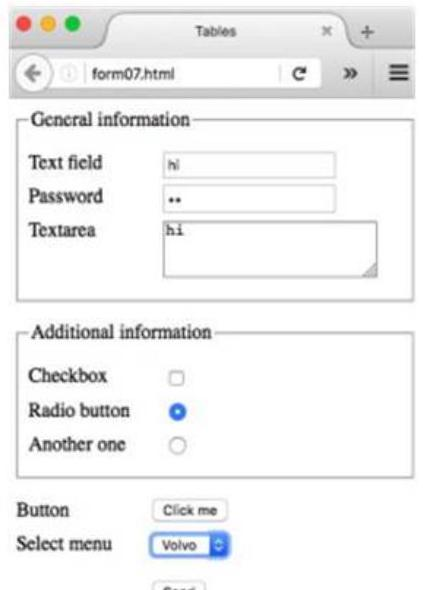
\includegraphics[width=\linewidth]{images/2024_12_29_858f09cde51177c71657g-29}
\end{center}

Formulare können auch POST/GET Aktionen ausführen:\\
Action beschreibt das Skript, welches die Daten annimmt. Method ist die Methode die ausgeführt wird.

\begin{lstlisting}[language=JavaScript, style=basesmol]
<form action="/login" method="post">
2 ...
3 </form>
\end{lstlisting}

\begin{center}
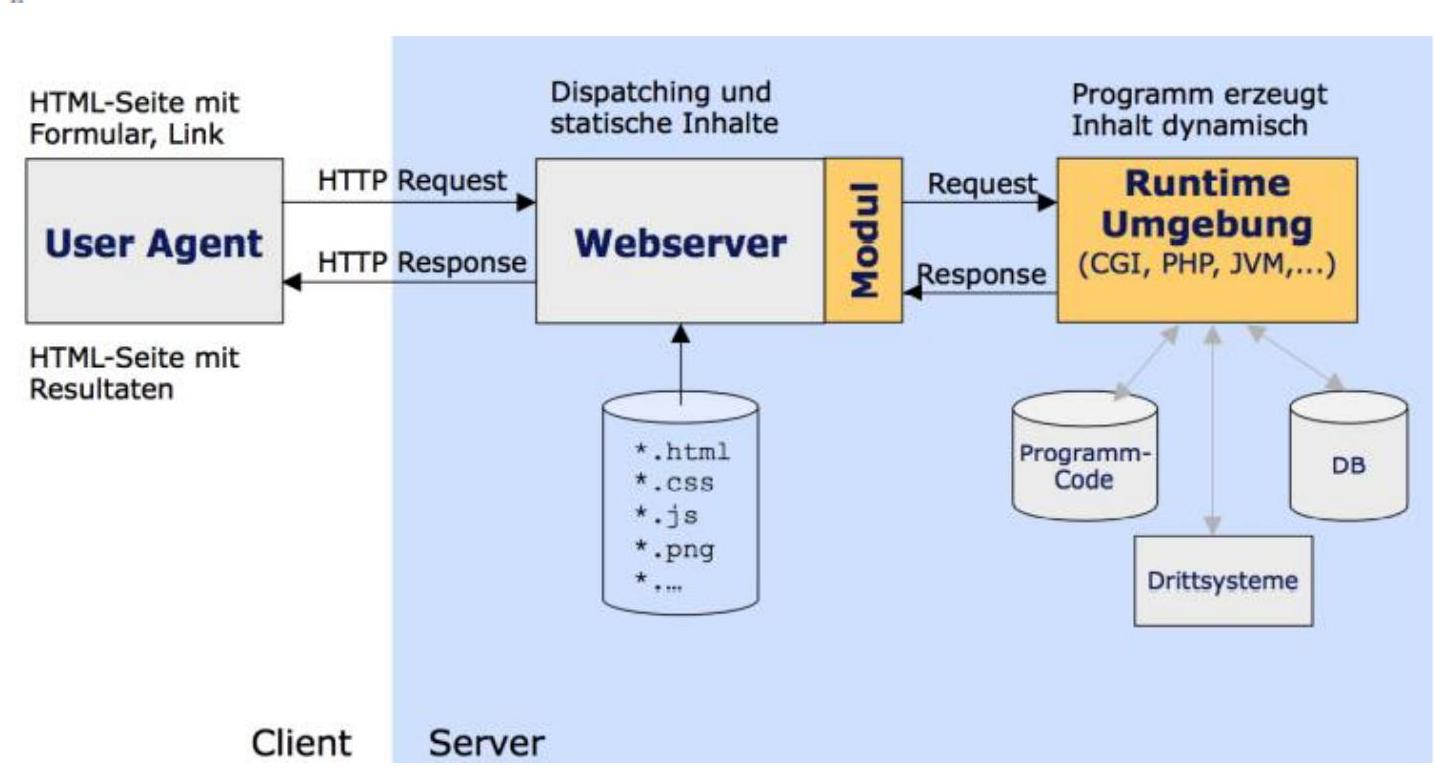
\includegraphics[width=\linewidth]{images/2024_12_29_858f09cde51177c71657g-29(1)}
\end{center}

Formular Events\\
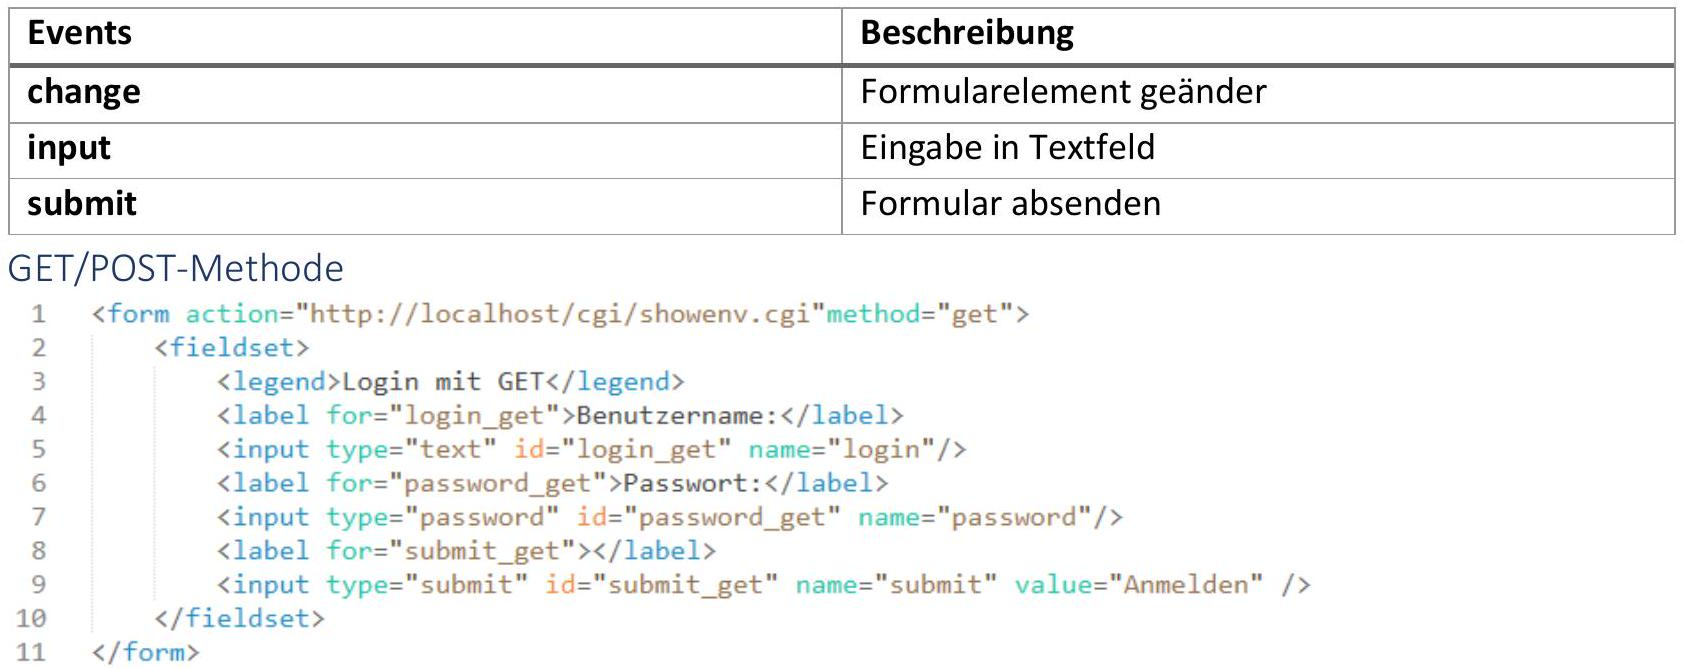
\includegraphics[width=\linewidth]{images/2024_12_29_858f09cde51177c71657g-30}

\subsubsection{Event Handling für Formulare}
\begin{definition}{Default-Verhalten}
Das Default-Verhalten von Formularen kann mit \texttt{preventDefault()} unterbunden werden.
\begin{lstlisting}[language=JavaScript, style=basesmol]
let form = document.querySelector("form");
form.addEventListener("submit", event => {
    event.preventDefault();
    console.log("Formular abgesendet!");
});
\end{lstlisting}
\end{definition}

\subsection{Cookies und Sessions}

\begin{definition}{Cookies}
Cookies speichern clientseitig Daten:
\begin{lstlisting}[language=JavaScript, style=basesmol]
document.cookie = "username=Max; expires=Fri, 31 Dec 2025 23:59:59 GMT";
console.log(document.cookie);
\end{lstlisting}
\end{definition}

\begin{definition}{Sessions}
Sessions speichern serverseitig Daten und nutzen eine Session-ID für die Zuordnung:
\begin{lstlisting}[language=JavaScript, style=basesmol]
// Beispiel: Session-Handling mit Express.js
req.session.user = "Max";
console.log(req.session.user);
\end{lstlisting}
\end{definition}

\begin{definition}{Cookies}

\begin{itemize}
\item HTTP als zustandsloses Protokoll konzipiert
\item Cookies: Speichern von Informationen auf dem Client
\item Response: Set-Cookie -Header, Request: Cookie -Header
\item Zugriff mit JavaScript möglich (ausser HttpOnly ist gesetzt)\\
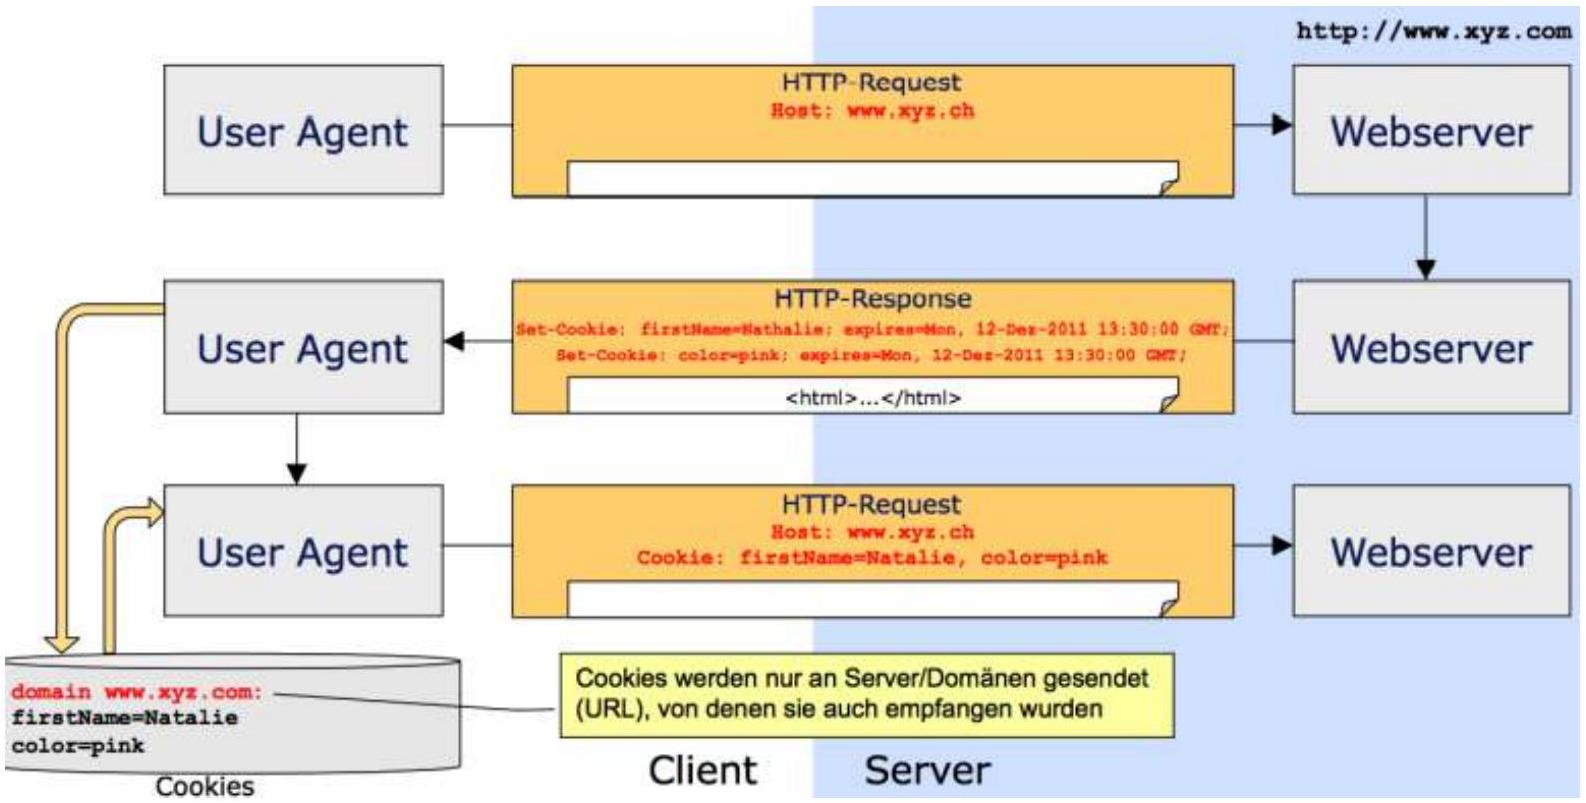
\includegraphics[width=\linewidth]{images/2024_12_29_858f09cde51177c71657g-31}
\end{itemize}
\end{definition}

\begin{definition}{Sessions}
\begin{itemize}
\item Cookies auf dem Client leicht manipulierbar
\item Session: Client-spezifische Daten auf dem Server speichern
\item Identifikation des Clients über Session-ID (Cookie o.a.)
\item Gefahr: Session-ID gerät in falsche Hände (Session-Hijacking)
\end{itemize}
\end{definition}
Ablauf:\\
\href{http://www.xyz.com}{http://www.xyz.com}\\
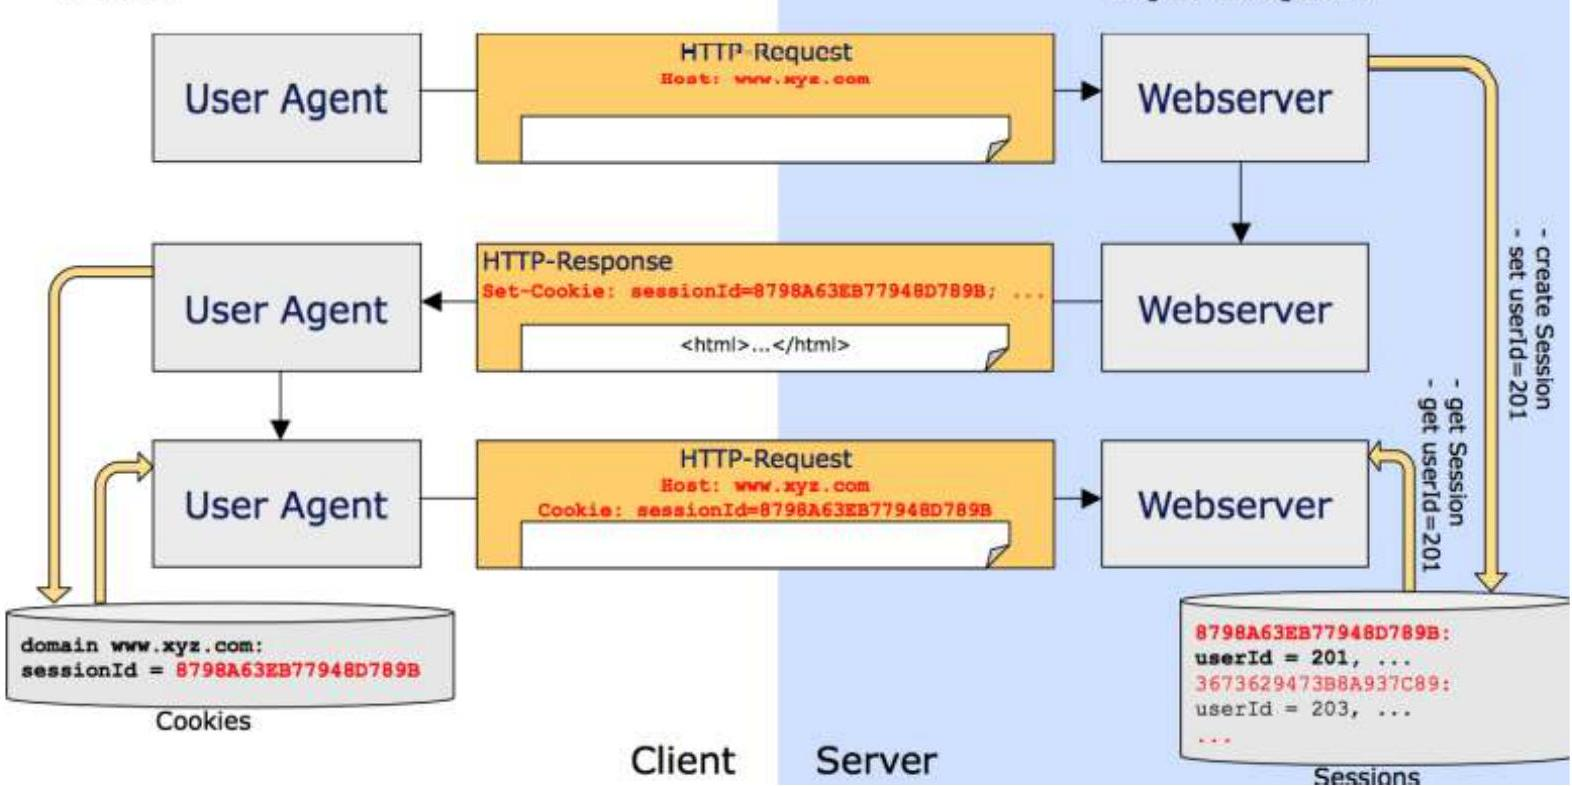
\includegraphics[width=\linewidth]{images/2024_12_29_858f09cde51177c71657g-31(1)}


\subsection{Fetch API}

\begin{definition}{Fetch API}
Mit der Fetch-API können HTTP-Requests ausgeführt werden:
\begin{lstlisting}[language=JavaScript, style=basesmol]
fetch("/data.json")
  .then(response => response.json())
  .then(data => console.log(data))
  .catch(error => console.error("Fehler:", error))
\end{lstlisting}
\end{definition}

\begin{definition}{Fetch API}
\begin{itemize}
\item HTTP-Requests von JavaScripts
\item Geben Promise zurück
\item Nach Server-Antwort erfüllt mit Response-Objekt
\end{itemize}
\end{definition}
\begin{lstlisting}[language=JavaScript, style=basesmol]
fetch("example/data.txt")
.then(response => {
          console.log(response.status) // -> 200
  console.log(response.headers.get("Content-Type")) // -> text/plain
})
.then(resp => resp.text())
.then(text => console.log(text))
// -> This is the content of data.txt
\end{lstlisting}

Response Objekt

\begin{itemize}
\item headers : Zugriff auf HTTP-Header-Daten Methoden get, keys, forEach , ...
\item status: Status-Code
\item json() : liefert Promise mit Resultat der JSON-Verarbeitung
\item text() : liefert Promise mit Inhalt der Server-Antwort
\end{itemize}